\documentclass[tikz,border=2pt]{standalone}
\usepackage{pgfplots}
\pgfplotsset{compat=1.18}
\usetikzlibrary{positioning}
\usepackage{helvet}
\renewcommand{\familydefault}{\sfdefault}
\definecolor{ieeecolor}{HTML}{042C53}
\definecolor{jrnlcolor}{HTML}{378ADD}
\definecolor{othercolor}{HTML}{B4B2A9}
\definecolor{confcolor}{HTML}{D98B3F}
\begin{document}
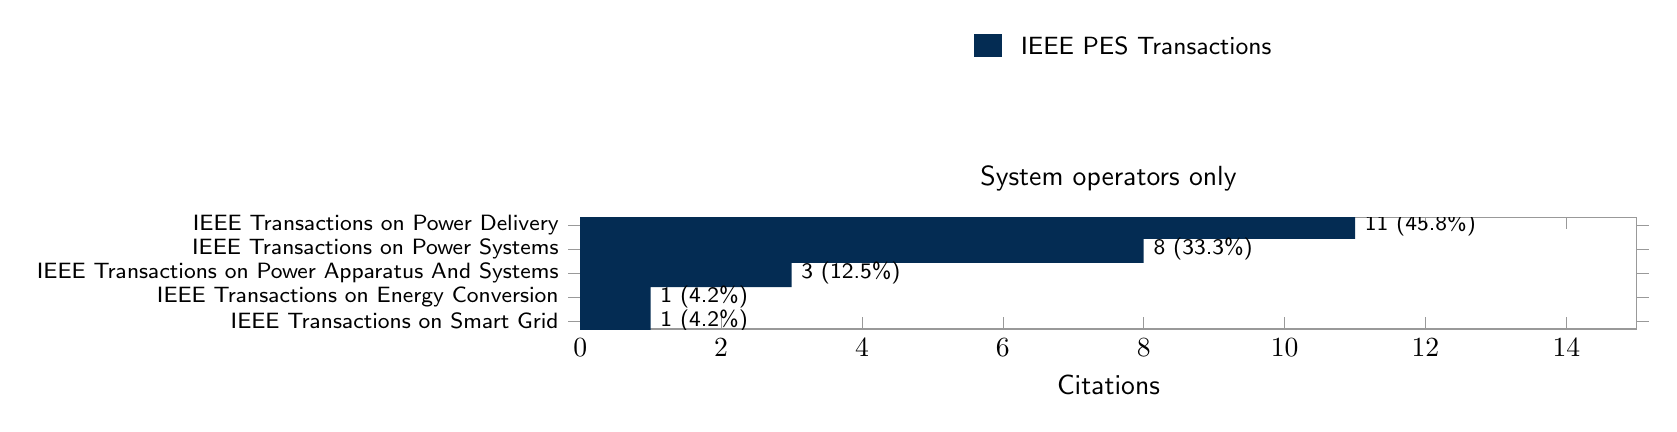
\begin{tikzpicture}
\begin{axis}[
    xbar, bar width=10pt, bar shift=0pt,
    width=15cm, height=3.0cm,
    symbolic y coords={IEEE Transactions on Power Delivery,IEEE Transactions on Power Systems,IEEE Transactions on Power Apparatus And Systems,IEEE Transactions on Energy Conversion,IEEE Transactions on Smart Grid},
    ytick=data,
    y dir=reverse,
    y tick label style={font=\footnotesize},
    xlabel={Citations},
    xmin=0, xmax=15,
    axis line style={color=black!40},
    tick style={color=black!40},
    enlarge y limits=0.08,
    title={System operators only},
]
\addplot[fill=ieeecolor, draw=none] coordinates {(11,IEEE Transactions on Power Delivery) (8,IEEE Transactions on Power Systems) (3,IEEE Transactions on Power Apparatus And Systems) (1,IEEE Transactions on Energy Conversion) (1,IEEE Transactions on Smart Grid)};
\node[anchor=west, font=\footnotesize] at (axis cs:11,IEEE Transactions on Power Delivery) {11 (45.8\%)};
\node[anchor=west, font=\footnotesize] at (axis cs:8,IEEE Transactions on Power Systems) {8 (33.3\%)};
\node[anchor=west, font=\footnotesize] at (axis cs:3,IEEE Transactions on Power Apparatus And Systems) {3 (12.5\%)};
\node[anchor=west, font=\footnotesize] at (axis cs:1,IEEE Transactions on Energy Conversion) {1 (4.2\%)};
\node[anchor=west, font=\footnotesize] at (axis cs:1,IEEE Transactions on Smart Grid) {1 (4.2\%)};
\end{axis}
\begin{scope}[shift={(5,3.6)}]
\node[fill=ieeecolor, minimum width=10pt, minimum height=8pt, anchor=west] (legbox0) at (0,0) {}; \node[anchor=west, font=\small, right=3pt of legbox0] (legtxt0) {IEEE PES Transactions};
\end{scope}
\end{tikzpicture}
\end{document}
